\documentclass[tikz,border=5pt]{standalone}
\usepackage[UTF8,fontset=fandol]{ctex}
\usepackage{amsmath,amssymb}
\usetikzlibrary{arrows.meta,calc}
\tikzset{every picture/.style={>=Latex,line cap=round,line join=round,font=\small},
 ray/.style={->,thick,blue!75!black},wall/.style={thick,black!80},
 guide/.style={dashed,thin,gray!65},
 optic/.style={draw=black!65,fill=blue!4,rounded corners=2pt,
 minimum width=.82cm,minimum height=.65cm,inner sep=4pt},
 source/.style={draw=black!60,circle,minimum size=.60cm,inner sep=1pt},
 axis/.style={->,semithick,black!75}}
\begin{document}

% 1. Unfolded channels; suffixes identify physical origin, both receivers are R.
\begin{tikzpicture}
 \foreach \yy/\src/\ps/\qs in {1.8/R/P_R/Q_R,0/L/P_L/Q_L}{
  \node[source](s\src)at(0,\yy){$\src$};
  \node[optic](p\src)at(1.55,\yy){$\ps$};
  \node[optic](q\src)at(3.10,\yy){$\qs$};
  \node[optic,fill=gray!12](m\src)at(4.65,\yy){$M$};
  \node[optic](u\src)at(6.20,\yy){$Q_R$};
  \node[optic](v\src)at(7.75,\yy){$P_R$};
  \node[source](r\src)at(9.30,\yy){$R$};
  \draw[ray](s\src)--(p\src);
  \draw[ray](p\src)--(q\src);
  \draw[ray](q\src)--(m\src);
  \draw[ray](m\src)--(u\src);
  \draw[ray](u\src)--(v\src);
  \draw[ray](v\src)--(r\src);
 }
 \node[above,align=center]at(0,2.23){源点};
 \node[above]at(2.32,2.23){向外：$P\to Q$};
 \node[above]at(4.65,2.23){反射};
 \node[above]at(6.98,2.23){向内：$Q\to P$};
 \node[above,align=center]at(9.30,2.23){右眼接收};
 \node[below]at(4.65,-.59){展开光路；老式镜片去掉各 $Q$};
\end{tikzpicture}

% 2. True transverse principal axes; neither optic axis is longitudinal.
\begin{tikzpicture}
 \draw[axis](-2.75,0)--(3.05,0)node[right]{$x,\ P_R$};
 \draw[axis](0,-2.45)--(0,2.70)node[above]{$y,\ P_L$};
 \draw[orange!75!black,thick,->](-1.90,-1.90)--(2.10,2.10)
  node[above right]{$a$};
 \draw[blue!70!black,thick,->](1.90,-1.90)--(-2.10,2.10)
  node[above left]{$b$};
 \draw[thin](.83,0)arc[start angle=0,end angle=45,radius=.83];
 \node at(1.23,.48){$45^\circ$};
 \filldraw(0,0)circle(1.3pt);
 \node[below]at(0,-2.75){片面内的电场方向};
\end{tikzpicture}

% 3. Fixed-space transverse field trajectory, no ray circle.
\begin{tikzpicture}
 \foreach \x/\name in {0/入射线偏振,4.4/单程圆偏振,8.8/双程线偏振}{
  \begin{scope}[xshift=\x cm]
   \draw[axis](-1.35,0)--(1.50,0)node[right]{$E_a$};
   \draw[axis](0,-1.35)--(0,1.50)node[above]{$E_b$};
   \node[above]at(0,1.91){\name};
  \end{scope}
 }
 \draw[blue!75!black,very thick](-.99,-.99)--(.99,.99);
 \draw[blue!75!black,very thick](4.4,0)circle(.99);
 \draw[->,blue!75!black,thick](5.39,0)arc[start angle=0,end angle=-65,radius=.99];
 \draw[blue!75!black,very thick](7.81,.99)--(9.79,-.99);
 \draw[ray](1.78,.22)--(2.75,.22);
 \draw[ray](6.18,.22)--(7.15,.22);
 \node[below,align=center]at(0,-1.77){$\Delta\phi=0$\\$y=(a+b)/\sqrt2$};
 \node[below]at(4.4,-1.77){$\Delta\phi=\pi/2$};
 \node[below,align=center]at(8.8,-1.77){$\Delta\phi=\pi$\\$x=(a-b)/\sqrt2$};
\end{tikzpicture}

% 4. Screen input direction is into the glasses, not the face's outward channel.
\begin{tikzpicture}
 \foreach \yy/\circ/\lin/\pass/\stop in {1.8/C_+/x/P_R/P_L,0/C_-/y/P_L/P_R}{
  \node[optic,minimum width=1.1cm](c\lin)at(0,\yy){$\circ$};
  \node[optic](q\lin)at(2.25,\yy){$Q$};
  \node[optic,minimum width=1.1cm](l\lin)at(4.50,\yy){$\lin$ 线偏振};
  \node[optic,fill=green!6,minimum width=1.75cm](p\lin)at(7.10,\yy){$\pass$ 通过};
  \draw[ray](c\lin)--(q\lin);
  \draw[ray](q\lin)--(l\lin);
  \draw[ray](l\lin)--(p\lin);
  \node[right]at(8.30,\yy){$\stop$ 阻挡};
 }
 \node[above]at(0,2.44){投影光};
 \node[above]at(2.25,2.44){外侧波片};
 \node[above]at(7.10,2.44){内侧验偏器};
 \node[below]at(4.25,-.63){入射：银幕 $\longrightarrow$ 眼睛};
\end{tikzpicture}

% 5. General phase; plotted only at chi=45 degrees. Both powers normalize after P.
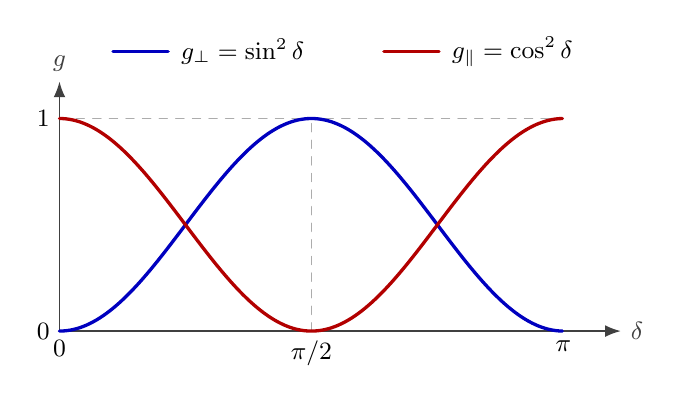
\begin{tikzpicture}
 \draw[axis](0,0)--(7.13,0)node[right]{$\delta$};
 \draw[axis](0,0)--(0,3.17)node[above]{$g$};
 \draw[guide](0,2.70)--(6.4,2.70);
 \draw[guide](3.2,0)--(3.2,2.7);
 \draw[blue!75!black,very thick,domain=0:1,samples=151]
  plot({6.4*\x},{2.7*(sin(180*\x))^2});
 \draw[red!70!black,very thick,domain=0:1,samples=151]
  plot({6.4*\x},{2.7*(cos(180*\x))^2});
 \node[left]at(0,0){$0$};
 \node[left]at(0,2.7){$1$};
 \node[below]at(0,0){$0$};
 \node[below]at(3.2,0){$\pi/2$};
 \node[below]at(6.4,0){$\pi$};
 \draw[blue!75!black,very thick](.68,3.55)--(1.38,3.55);
 \node[right]at(1.42,3.55){$g_\perp=\sin^2\delta$};
 \draw[red!70!black,very thick](4.12,3.55)--(4.82,3.55);
 \node[right]at(4.86,3.55){$g_\parallel=\cos^2\delta$};
\end{tikzpicture}

% 6. Spatial layer ordering; x direction is physical face -> external space.
\begin{tikzpicture}
 \foreach \idx/\yy/\lab/\first/\second in {A/1.8/正确层次/P/Q,B/0/反装层次/Q/P}{
  \node[left]at(0,\yy){\lab};
  \node[optic,minimum width=.75cm](eye\idx)at(.9,\yy){眼};
  \node[optic](first\idx)at(3.1,\yy){$\first$};
  \node[optic](second\idx)at(5.3,\yy){$\second$};
  \node[optic,fill=gray!12](outer\idx)at(8.0,\yy){外侧};
  \draw[ray](eye\idx.north east)--(first\idx.north west);
  \draw[ray](first\idx.north east)--(second\idx.north west);
  \draw[ray](second\idx.north east)--(outer\idx.north west);
  \draw[ray](outer\idx.south west)--(second\idx.south east);
  \draw[ray](second\idx.south west)--(first\idx.south east);
  \draw[ray](first\idx.south west)--(eye\idx.south east);
 }
 \node[above]at(1.0,2.45){脸部};
 \node[above]at(4.2,2.45){镜片内部 $\longrightarrow$ 前方};
 \node[above]at(8.0,2.45){镜面／银幕};
\end{tikzpicture}
\end{document}
